In this chapter we finally arrive at our main interest. First of all we introduce the hierarchy of data structures with respect to persistence.

\begin{itemize}
\item {\bfseries Ephemeral data structures} are the most widespread. 
Past states are destroyed by ``destructive” updates and irretrievably lost.
\item {\bfseries Semi-persistent data structures} (sometimes partially persistent) 
support queries on any version. It is only possible to update the most recent version, producing a new version. 
Historical versions form a linear order. 
\item {\bfseries (Fully-)persistent data structures} directly extend their semi-persistent counterparts. 
An update can be done on any version of the structure, resulting in a rooted tree of versions. 
An update corresponds to adding a new child version to an existing version in the tree.
\item {\bfseries Functional data structures} permit no changes to data once written. 
Naturally, persistence is guaranteed under such an assumption, 
as all versions appear as if just created by the last update.
This enforced immutability completely freezes past versions in time.
This concept is intrinsic to functional languages such as Haskell, 
but it proves to be useful even in imperative programming. 
Multi-threading is easier when there is confidence that existing objects will not be modified.
\end{itemize}

This division is by no means universally adopted, but it provides an interesting perspective regardless.

With a persistent data structure, we essentially want to have one data structure for every existing version. 
Insert and delete return a new version handle instead of making changes to the existing version. 
Obviously, copying the data structure every time is one option how to achieve this, albeit not a great one. 
To prevent using extra memory and increased time complexity of operations, more intricate methods must be employed.

Going beyond this hierarchy, if fully-persistent data structure also supports merging or melding two different versions, it is said to be \emph{confluently persistent}. 
Confluently persistent data structures are the subject of studies for example by Driscoll, Sleator, and Tarjan \cite{confluently-persistent-a} or Fiats and Kaplan \cite{confluently-persistent-b}. 
We will not investigate confluent persistence further in this thesis.

Driscoll et al.~\cite{persistence-DSST} developed a framework for persistence of pointer-based data structures. 
Some of the techniques which we will use will be nearly identical to those of Driscoll et al.
We limit ourselves to the context of binary search trees. 
Nonetheless, the algorithms typically naturally generalize to other kinds of pointer-based data structures.


\section{Persistence through path-copying}

Let us open with a few simple constructions first. A binary search tree can be converted into a fully-persistent one rather easily.
The straight-forward approach is called path-copying. It is based on the observation that most of the tree does not change during an update.

When a new version of the tree should be created by delete or insert, new copies are allocated only for vertices that are changed by the operation, and for their ancestors. 
This typically means that only the path from the inserted/deleted vertex to the root is newly allocated, plus a constant number of other vertices. 
The new vertices carry pointers to the old vertices where the subtree rooted at such a vertex is not modified in any way.
As the root is changed by every update, it is used to represent its version of the data structure.

Here we tacitly assume that only pointers to children are stored. 
Updating root in a tree with pointers to parents would involve creating new instances for all nodes in the tree.

With reasonable variants of binary search trees, achieved time complexity in a tree with $n$ vertices is $\Theta(\log n)$ per operation and $\Theta(\log n)$ memory for one insert/delete is needed.

The downside of this method is the increased space complexity. 
There is no apparent construction that would not increase memory complexity by copying the paths.

\section{Multiple versions in one vertex}

To limit memory consumption we may rather choose to let vertices carry their properties for all versions. This in reality means that we must store a collection of changes together with versions when those changes happened. This makes a vertex a kind of dictionary with keys being versions and values the descriptions of changes.

When semi-persistence is sufficient, upon arriving at a vertex asking for the state in version $A$, we do the following: We must go through the collection of changes to figure out what values of pointers and fields are valid for version $A$. 
We start with the default values and apply all changes that happened earlier than $A$ in chronological order. When a  overwriting if there are multiple changes for the same field or pointer. 
This process yields the correct state of the vertex for version $A$. 

In fact, it might be easier to just copy all the other fields the vertex possesses as well if one of them changes.
One change will therefore hold new values for all fields and pointers of the vertex. 

For full persistence we also need to resolve the issue of how to efficiently determine which changes should be applied. 
It will be addressed later through introduction of total ordering of all versions.

Looking at the memory consumption, it appears clear that the amount consumed stems from the total number of changes done by the balancing algorithm across all operations.

What remains to solve though is to choose the right kind of data structure for versions of changes for one vertex. Surely using linked lists or arrays will inevitably lead to unsatisfactorily inefficient processing of applicable changes. Unfortunately as it turns out, even other data structures will let us down.

With this approach, we can reach space complexity that is linear with the total number of changes in the tree. On the other hand, execution time will be hurt. We can reach the following amortized complexity depending on the chosen data structure:\\

\begin{tabular}{ll}
Linked list & \bigO{n \log n} \\
Binary search tree & \bigO{\log^2 n} \\
Q-fast trie \cite{q-fast-trie} & \bigO{\log ^{3/2} n}, semi-persistence only \\
Y-fast trie \cite{y-fast-trie} & \bigO{\log n \cdot \log \log n}, semi-persistence only, on average

\end{tabular}

\begin{figure}
	\begin{center}
		\begin{tikzpicture}[sibling distance=8pt]
		\Tree[
		.B A [ .C \edge[blank]; \node[blank]{}; D ]
		]
		\node at (0,1) {Version 1};
		\end{tikzpicture}
		\qquad\hspace{40mm}
		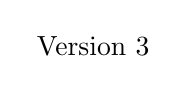
\begin{tikzpicture}[sibling distance=8pt]
		\Tree[
		.B A [ .D C E ]
		]
		\node at (0,1) {Version 3};
		\end{tikzpicture}
	\end{center}
\raggedcolumns
\begin{multicols}{2}
\centering
\footnotesize
\begin{vdTable}{Vertex}
	Version & Left & Right   & Key & Value
\end{vdTable}
\begin{vdTable}{A}
	1 & $\Lambda$ & $\Lambda$ & 10 & 5 \\
	2 & $\Lambda$ & $\Lambda$ & 10 & 6
\end{vdTable}
\begin{vdTable}{B}
	1 & A & C & 20 & 15 \\
	3 & A & D & 20 & 15
\end{vdTable}
\begin{vdTable}{C}
	1 & $\Lambda$ & D & 30 & 27 \\
	3 & $\Lambda$ & $\Lambda$ & 30 & 27
\end{vdTable}
\begin{vdTable}{D}
	1 & $\Lambda$ & $\Lambda$ & 40 & 39 \\
	3 & C & E & 40 & 39
\end{vdTable}
\begin{vdTable}{E}
	3 & $\Lambda$ & $\Lambda$ & 50 & 99
\end{vdTable}\\
\end{multicols}

{\small
Tree is shown for version 1 (left) and 3 (right). 
Internal collections for each vertex are displayed. 
Operation that created version 2 changed value of key 10. Operation that created version 3 inserted vertex E and triggered a rotation. 
Faithful to The Art of Computer Programming, $\Lambda$ represents a null pointer.
}

\caption{A tree with dictionaries in vertices} 

\end{figure}

\section{Fat vertices}

Following up on the idea of multiple versions in one vertex, fat vertices were devised. 
We will explain this technique only for semi-persistence first. 
Full persistence requires the use of a few extra tricks and establishing an ordering on the versions.

A \emph{fat vertex} stores a collection of standard vertices indexed by versions. 
We call values of this collection \emph{slots}. 
The maximum size of this dictionary is set to a constant which is to be determined later. 
Temporarily, we will allow the capacity of a fat vertex to be exceeded. 
This will have to be fixed however, before the ongoing operation finishes.
By placing a restriction on the size we may circumvent the increased complexity of search within one vertex.
Instead of copying the vertex, we simply add a new slot into the dictionary. 
Provided the maximum has not been exceeded yet, this insertion of a slot stops the propagation of changes toward the root. 
The reader should recall that this propagation was the major weakness of path-copying.
Because of the limit on size of this dictionary, it may be implemented simply as a linked list.

Contents of one slot are a version handle, all pointers a vertex would have, then inverse pointers to fat vertices that have slots pointing to this fat vertex for this version and some fields, notably key and value as a bare minimum.
Not all fields need to be versioned. 
For example balancing information may be stored only for the latest version, i.e, in a red-black trees color is only used for balancing and is thus not needed to be persisted for old versions. 
(Until full-persistence comes into play.)

One vertex in the original binary search then corresponds to a doubly-linked list of fat vertices.
When the vertex changes, a new state of the vertex is written into a slot of the last fat vertex in the list. 
As all slots become occupied in the last fat vertex and it needs to be modified, new vertex is allocated.

Modifications of a single vertex during one operation are all written to single slot, there is no need for using more slots.

We will need to be able to determine for any fat vertex $x$ which other fat vertices have their most recent slot pointing to $x$. 
This problem is resolved by adding some number of \emph{inverse pointers} to vertices. 
We define an invariant of inverse pointers: If vertex $v$ points to vertex $u$ in version $\alpha$, then $u$ in version $\alpha$ contains an inverse pointer to $v$. This invariant is maintained by also changing the inverse pointers whenever some proper pointers change. 

When a new fat vertex $x$ is allocated, one of its slots is immediately taken. 
Pointers must be updated in other fat vertices whose latest slot  pointed to the fat vertex preceding $x$ in the list. 
This is done by going through inverse pointers and either creating slots (copying all values from the latest slot and replacing pointers to the predecessor by pointers to $x$), or directly updating the pointers if the slot for the right version is already present. 
Also, we need to go through proper pointers and update inverse pointers in other fat vertices in a similar fashion.

Recursive allocations may be triggered, which is not a problem if there is only a small amount of them. 
This is ensured by setting the size of fat vertices suitably. 
The order in which these allocations are executed can be arbitrary.
We can place an upper bound on the number of newly allocated fat vertices -- total number of vertices in the tree (including deleted vertices). 
At most one new slot is occupied for every vertex in the tree.

To take advantage of fat vertices, we need the balancing algorithm to limit the number of vertices that change in one operation. 
It is sufficient that the changes can be amortized to a constant number per update, ideally it should be a constant even in the worst case.
This was the goal of modified WAVL-balancing algorithm all along. 
Furthermore, we need a limit on the number of pointers that can target one vertex at one time.

\begin{prop}
Consider any binary search tree balancing algorithm satisfying the following properties:
\begin{itemize}
\item 
There is a constant $d$ such that for any $n$ successive operations on an initially empty tree, the number of vertex changes made to the tree is at most $dn$. 
\item 
There is a constant bound on the number of pointers to any one vertex at any time.
\end{itemize}
Then this algorithm with the addition of fat vertices for semi-persistence, consumes \bigO{n} space for the entire history of $n$ operations starting from an empty tree.
\end{prop}

\begin{myproof}
We denote the number of pointer fields per vertex by $p$ and the maximum number of vertices pointing to one vertex at a time by $k$. 
We then define the number of slots in one fat node as $s = p + k + 1$ and add $k$ inverse pointers to vertices.

We define the potential of the structure as the total number of occupied slots in all fat vertices that are the last in their doubly-linked list. 
(Thus initially zero.) 
Allocation of a new fat vertex will cost one unit of energy. 
This cost can be paid from the potential or the operation. 
We will show that the operation needs to be charged only a constant amount of energy per one vertex modification by the original algorithm (to compensate for the increase in potential or to pay for allocations), from which the proposition follows.

For insert, a new fat node is created with one occupied slot and one slot is occupied in the parent of the newly created vertex (which increases potential by a constant). 
This increase is paid for by the operation. During rebalancing of the tree, $r$ vertices are to be modified. 
The situation is similar for delete.
Let us consider this sequence of modifications one by one. 
The operation sends one floating unit of energy to each of the $r$ vertices.

If a modification of $v$ is second or later modification of $v$ during an ongoing update, changes are simply written to the slot for the created version. 
Otherwise, the number of used slots is checked. 
If there is one or more empty slots available, one of the is used. 
The new slot takes values of unchanged fields and pointers from the preceding slot. 
This increases the potential by one, which is covered by the floating unit of energy.

If no slots are available, new fat vertex $v'$ is allocated and one of its slots is used. 
This step triggers a decrease in the potential by $p+k$. 
The floating unit of energy is used to pay for allocation of the new vertex. 
Next, fat vertices to corresponding current version interval of vertices having pointers to $v$ need to have this reflected. 
Additionally, inverse pointers to $v'$ need to be set. 
These are at most $p+k$ changes to other vertices that may use their new empty slots. 
The decrease in potential is used to send one unit of energy to every such vertex that need an update. 
Changes are executed recursively and will not require extra energy to be charged on this modification.

The operation is charged only constant amount of work for every change it does.
Space complexity consumed is bounded by the number changes done by update operations. Thus space complexity is \bigO{n}. 
\end{myproof}

Regarding the time complexity, searching the correct slot in a fat vertex produces only constant overhead. Realizing that every operation can be charged on a memory allocation of a fat vertex such that there is a constant $c$ depending only on the balancing algorithm such that for every allocated fat vertex the number of operations charged on it is at most $c$.

\begin{obs}
Assuming the conditions from the previous proposition, the cost to write changes into fat vertices is amortized to \bigO{1} per operation.
\end{obs}

We see that WAVL trees can be used for semi-persistence even in their original form, along with many other binary search trees. Time complexity of operations with the tree depends on the original balancing algorithm used. With WAVL trees we get \bigO{\log n} per operation from the original algorithm in addition to the amortized \bigO{1}. Here $n$ is the size of the tree in the version that is queried.

In fact, for semi-persistence fat vertices may be defined differently. It suffices that only values of changed fields and pointers are written into slots. 
Thus each fat vertex carries a set of default values for every field and pointer, these values are used if not overridden by a slot. 
This approach may lead to lower memory consumption, but it is not directly compatible with the approach to full persistence described later.

\begin{figure}
\begin{center}
	\ttfamily
	\begin{tabular}{cccccc}
		Rank  & Previous &  Next   &      & &          \\ \hline
		Left1 &  Right1  & Parent1 & Key1 & Value1 &  Version1 \\ \hline
		Left2 &  Right2  & Parent2 & Key2 & Value2 & Version2 \\ \hline
		Left3 &  Right3  & Parent3 & Key3 & Value3 & Version3 \\ \hline
		Left4 &  Right4  & Parent4 & Key4 & Value4 & Version4 \\ \hline
		Left5 &  Right5  & Parent5 & Key5 & Value5 & Version5 \\ \hline
		Left6 &  Right6  & Parent6 & Key6 & Value6 & Version6 \\ \hline
	\end{tabular}
\end{center}
Rank of WAVL trees is not used for navigation, only for balancing the tree. So it need not be maintained for older versions.
\caption{Layout for WAVL semi-persistent tree fat vertex}
\end{figure}

\section{Parallel Semi-persistence with WAVL trees}

In this section we explore the potential of semi-persistent WAVL trees as a parallel data structure. 
We begin by issuing a lock to every fat vertex.

Recall that insertion and deletion in a WAVL tree can be also carried out top-down.
By preemptively performing rotations, promotes and demotes when descending, we can make sure that large number of changes of vertices with high ranks will not be needed. This means that as insert or delete will descend down the tree towards the leaves processing vertices along some vertical path, it will hold locks for vertices in at most constant distance from the vertex that the operation is currently processing.

Also recall that there are at most \bigO{1} modifications of the structure per update (amortized), albeit the constant proves to be rather high. These facts lay a solid foundation to parallel semi-persistence.

What seems a bit unfortunate, is the delete procedure, which must locate an additional vertex to swap values in case of the deleted vertex having two children. So we will assume that delete is not possible for now.

First of all two kinds of supported operations must be identified. 

\begin{itemize}
	\item Query on any version of the tree (i.e., find, minimum, maximum and range functions)
	\item Insert (into the newest version of the tree)
\end{itemize}

Let us address data races between inserts first. For every insert, prior to all else, a new version handle must be created. This is achieved simply by incrementing a version counter which is done by a primitive such as fetch-and-add and will not block other threads. The insert itself follows.

To ensure that the most recent fat vertex for root does not change after some update starts waiting for the lock for access to it, we introduce additional \emph{latest-root} pointer. It must always point to the current latest fat vertex of the root for the most recent version. 

New updates start by waiting for lock for latest-root pointer. This lock is lifted when the holding operation wows not change root of the tree. When some update changes the fat vertex that corresponds to the root, it also updates latest-root pointer.

When we enter a fat vertex, we lock it for other threads of computation. Conversely, a lock for a fat vertex is lifted when it ceases to be in the subtree of current safe-node's parent for insert holding the lock. Since all threads begin locking at the root and descend towards the leaves, no deadlocking is possible among inserts. This follows from the fact that rotations may only be done among vertices locked by the same operation.

Applying the algorithm with semi-persistence we must additionally ensure that before unlocking a fat node, none of its children may run out of slots leading to allocation of a replacement. Since there can be at most one new slot occupied for every fat node in one operation, it suffices to allocate new fat vertex for every fat vertex without empty slots before releasing its parent. This may involve increasing the capacity of fat vertices.

To address queries, we assume that queries are only started on a version that was generated by an already complete insert. In this situation, queries may pass through fat vertices with little regard to ongoing inserts. Queries will thus ignore locks on fat vertices. 

Modification of slots currently processed by queries needs to be prevented. We can decide to add locks also to slots. Modification of slots by insert (being non-atomic) requires an exclusive write lock on the slots that are modified. Queries will require a shared read-only lock. Since reading of information from slots by insert may only be obstructed by writing in the same insert, the read-only lock is not needed in this case. No deadlocks will arise from this locking. It can be conducted starting from the first item in the list of slots in all cases. 

There is arguably a better solution though. The version of slots might be set atomically by updates as the last field to be set in creation of the slot. Query operations might check version of a slot first and if it is equal to the default value, assume that it is not yet occupied. This would indicate that all remaining slots are also empty. The query would thus know it does not need the information stored in those slots and proceed as if those did not exist. 
In this case memory barriers would be needed to ensure that all other fields and pointers are written before the version.

If we increase the number of slots in a fat vertex by at least one, asymptotic memory consumption remains linear with length of history. Time complexity for one operation remains the same as without this modification for concurrence, that is if the time spend being blocked by other threads is excluded.

Let us turn back to enabling delete. If delete operations are rare, we may simply treat them as inserts locking-wise and acknowledge that blocking may ensue. Another approach would be to use the technique of \textit{ghost vertices}. That is to add a deleted flag to vertex layout, deleting would simply set this flag in corresponding slot. This will increase size of the tree. For the number of deleted vertices bounded by a polynomial in the number of remaining vertices for every version of the data structure, this preserves the asymptotic time complexity. 

Otherwise, an entirely new data structure may be built from the latest versions of all vertices in the tree if the amount of deleted vertices exceeds a certain ratio to remaining vertices. The cost to build this new tree is amortized into the deletes from the preceding data structure.

\begin{figure}
	\begin{center}
		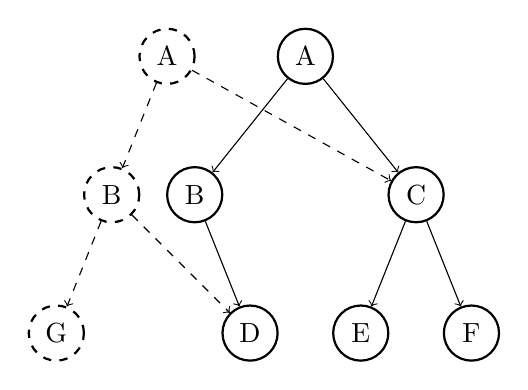
\begin{tikzpicture}[
			oldnode/.style={circle, draw=black, thick, minimum size=7mm},
			newnode/.style={circle, thick, draw=black, dashed, minimum size=7mm},
			]
			\node[oldnode] at (0,0) (root) {A};
			\node[oldnode] at (-4em,-5em) (beta) {B};
			\node[oldnode] at (4em,-5em) (gamma) {C};
			\node[oldnode] at (-2em,-10em) (delta) {D};
			\node[oldnode] at (2em,-10em) (epsilon) {E};
			\node[oldnode] at (6em,-10em) (zeta) {F};
			\node[newnode] at (-5em,0) (newroot) {A};
			\node[newnode] at (-7em,-5em) (newbeta) {B};
			\node[newnode] at (-9em,-10em) (newvertex) {G};
			\draw[->] (root) -- (beta);
			\draw[->] (root) -- (gamma);
			\draw[->] (beta) -- (delta);
			\draw[->] (gamma) -- (zeta);
			\draw[->] (gamma) -- (epsilon);
			\draw[->,dashed] (newroot) -- (gamma);
			\draw[->,dashed] (newroot) -- (newbeta);
			\draw[->,dashed] (newbeta) -- (newvertex);
			\draw[->,dashed] (newbeta) -- (delta);
		\end{tikzpicture}
	\end{center}
	A new vertex G was added to the structure with solid vertices. Dashed vertices were created by the update -- path from G to the root. Dashed A is the new root.
	\caption{Path-copying}
	\label{fig:path-copying}
\end{figure}

\section{List ordering}

Moving from semi-persistence to full-persistence we encounter an obstacle -- versions no longer form implicit linear order. (By versions we mean states of the tree in between updates. We will also use some auxiliary versions not directly mappable to any such state.) Nonetheless, to work with fat vertices, we need to be able to determine slots that carry values correct for current version. To achieve this, we need to identify an interval of versions the current version would fall into. For this purpose we will try to introduce an ordering to versions of the persistent data structure.

Version do form a rooted tree with the original version in the root. We can also order children of every vertex by the order of their creation (latest creation first). We then define the desired ordering as the order of vertices corresponding to versions as they are visited by an in-order traversal. %TODO: Reformulate in-order.

In reality, we will also insert other elements into the ordering that will be helper version and will not be used to represent the state of the entire structure after a sequence of operations. This can be disregarded for now.

With the ordering defined, we still need a way to efficiently represent it in memory. The operations we really need are two:

\begin{itemize}
	\item \texttt{InsertSuccessor(Version)} -- this operation will insert a new version between \texttt{Version} and its successor (if any). The newly created version is returned.
	\item \texttt{Compare(VersionA, VersionB)} -- returns 1, $-1$, or 0 indicating whether \texttt{VersionA} precedes, succeeds, or equals \texttt{VersionB}.
\end{itemize}

We will strive to find a way to assign an integer to each version, these integers will be comparable in constant time. This assignment problem is called \emph{list-labeling} and there are several options to tackling it.

The straight-forward idea would be to assign 0 to the first version and $2^m$ to an artificial upper bound. All newer versions will be assigned the arithmetic average of its successor and predecessor. Now, we see that if $v = (p + s)/2$ and $ 2^k \mid p, s$, then $2^{k-1} \mid v$. The first two integers are divisible by $2^m$ guaranteeing capacity $\Omega(m)$. 

Let us denote the total number of updates to the persistent tree as $n$. It would be reasonable to  assume that arithmetic operations on non-negative integers less than or equal to $n$ can be done in constant time. We are therefore permitted to create only \bigO{\log n} versions using the straight-forward idea if constant time per operation is needed. This is not sufficient.

To preserve the speed of semi-persistence, \texttt{Compare} must be \bigO{1} and \texttt{InsertSuccessor} \bigO{\log n} at least amortized. Weight-balanced trees that were introduced in the previous chapter are ideally suited for this purpose.

For every vertex in the weight-balanced tree, we will store encoding of the path from root to it in form of sequence of 0s and 1s. 1 for right child, 0 for left child. We know that depth of the tree must be logarithmic, compared integers are composed of \bigO{\log n} bits, so comparison of versions is efficient. Inserting a successor version is also simple. Rebuilding of some subtree will not change order of versions as all path encodings will be recalculated.

Before moving to the next section, we remark that it is possible to get \bigO{1} amortized complexity for insert and delete with weight-balanced trees via indirection as described by Tsakalidis \cite{list-ordering}.

\section{Fully-Persistent trees}

Before delving into the details of modified fat vertices for full-persistence, we must note that amortized constant number of changes per operation will no longer suffice. If there exist a version of the structure and an operation that causes large amount of changes to the structure, nothing is stopping us from repeatedly performing the operation on that version, thus consuming super-linear amount of space, (Potentially even time complexity may increase.)

To achieve full persistence, we will build upon the technique of fat vertices from previous sections. All pointers and fields will need to be versioned this time. Now however, simply allocating new vertex when we run out of empty slots in the old one will not do. It remains crucial that occupied slots of one fat vertex form an interval of existing versions. In particular, It will be needed to insert between existing versions.

Fat nodes of one vertex in the tree will be linked into a list in the order of increasing version-intervals that those fat nodes represent. A new maximum size $m$ of fat vertices will have to be set. If $p$ is the number of pointer fields in original vertices and $k$ the number of required inverse pointers, we set $m = 2(p+k+1)$.
When searching a fat vertex, the slot that applies has the greatest version not exceeding the version that is currently being searched for.

A process modifying the BST data structure may be broken down into a series of updates that only change one vertex or insert a new one. A deleted vertex is not reachable from the root, but technically still exists.
Every such update of the data structure will produce a new version (more than one typically). Since we were are only interested in the versions that are associated with the modification that completed an operation on the data structure, existence of other versions can be safely ignored. The total number of versions created will still be in linear with the number of total operations, preserving time complexity.

The process of performing one update involves first of all locating the slot that will be updated. If there exists a slot with the exact same version $v$, it will be updated. Otherwise the slot $s$ corresponding to $v$ is located and copied twice, creating slots $s'$ and $s''$. Slot $s'$ is given the version $v$ and $s''$ a newly created version that succeeds $v$. Then values in $s'$ are updated.
If the update is insert, a new fat vertex with one slot is created instead and its field and pointer values are initialized.

All inverse pointers must be updates accordingly. Either directly if version of their slots match, or by using the addition of two do/undo slots as explained. Of course this addition of slots may have exhausted the capacity of some fat nodes. We see however that at most constant number of slots was added altogether. 

We now need a process to somehow split the fat nodes which are over their capacity. Intuitively, for every fat node $f$ in excess of its capacity we would like to create a new fat node $f'$ and insert it after $f$ into the list of fat nodes for the same vertex. Then it would be possible to redistribute slots in $f$ between $f$ and $f'$ equally while preserving the invariant that fat nodes correspond to an interval of versions. Of course, when we do the splitting, we need to update pointers to $f$ in other vertices if they fall into the interval covered by $f'$.

This is roughly what the process will be. Unfortunately, when we split a fat node, some slots in other vertices may suddenly correspond to versions in both $f$ and $f'$. Pointer $t$ in a slot $s$ is called \emph{overlapping} if $s$ represents more versions than the fat node pointed to by $t$.
From the interval property of slots, this may happen for at most one slot $o$ in a vertex. We can solve this by inserting a new slot after $o$ with version of $f'$ and values equal to those of $o$ except the one problematic overlapping pointer which will point to $f'$.

Naturally, this insertion of slots may cause other fat nodes to exceed their capacity. What is worse, when fat nodes grow beyond constant size, complexity will suffer. There seems to be no clever method of selecting the next node to be split without the potential of some fat nodes growing beyond \bigO{1} before coming to be split. We therefore choose to delay the insertion of slots that correct overlapping pointers.

The full process for invariant maintenance follows. (The reader may see some similarities with the concept of fractional cascading.) We maintain a list $l$ of fat nodes, all vertices modified in this update are added to it. Until $l$ is not empty, we extract a vertex $w$ from $l$ and do the following steps with it:

\begin{itemize}
\item {\bf Removal of overlapping pointers.} Going from the slot with the lowest version to the highest, we identify overlapping pointers. From the logic of this algorithm, overlapping pointer $r$ always point to the first fat node representing versions contained in the slot of $r$. 

When an overlapping pointer $q$ is found, we schedule an addition of a slot. This new slot should be inserted when we reach the place inside the list of slots where $q$'s fat node's interval of versions ends. This new slots takes the rest of pointers and fields from its predecessor. (We can have an insertion scheduled for all types of pointers at the same time.) If there are still some versions remaining to be covered from $q$'s original interval, another addition of a slot is scheduled.

\item {\bf Allocation of new nodes.} If capacity of $w$ is not exceeded, continue with processing the next vertex in $l$. Otherwise, We set $x$ equal to the number of slots in $w$ divided by $m$ rounded down. Then we distribute slots evenly between $w$ and $(x-1)$ new fat vertices which are linked after $w$ into the list of fat nodes for this vertex.

\item {\bf Identification of overlapping pointers.} We now inspect all fat nodes pointed to by newly created fat nodes in previous step. We look at the pointers to those new vertices, we correct those pointers to point to the first fat node $t$ in the with $w$ such that there is an intersection of the versions represented by $t$ and the slot containing this pointer.

All fat nodes that were identified to contain an overlapping pointer must be added to $l$ if not added already.
\end{itemize}

\begin{figure}
\def\vl#1{\draw[color=black,dashed] (#1,0) -- (#1,3);}
\begin{center}
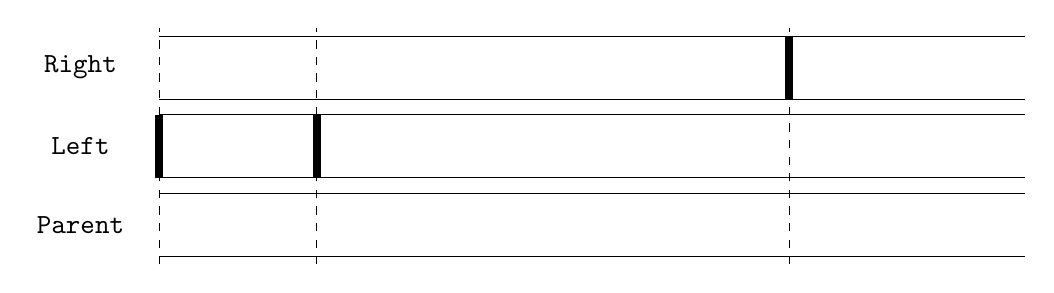
\begin{tikzpicture}
	\draw (0,2.9) -- (11,2.9);
	\draw (0,2.1) -- (11,2.1);
	\draw (0,1.9) -- (11,1.9);	
	\draw (0,1.1) -- (11,1.1);
	\draw (0,0.9) -- (11,0.9);
	\draw (0,0.1) -- (11,0.1);
	
	\vl{0}
	\vl{2}
	\vl{8}
	
	\draw[line width = 1mm] (0,1.1) -- (0,1.9);
	\draw[line width = 1mm] (2,1.1) -- (2,1.9);
	\draw[line width = 1mm] (8,2.1) -- (8,2.9);
	
	\node at (-1,0.5) {\tt Parent};
	\node at (-1,1.5) {\tt Left};
	\node at (-1,2.5) {\tt Right};
\end{tikzpicture}
\vspace{10mm}

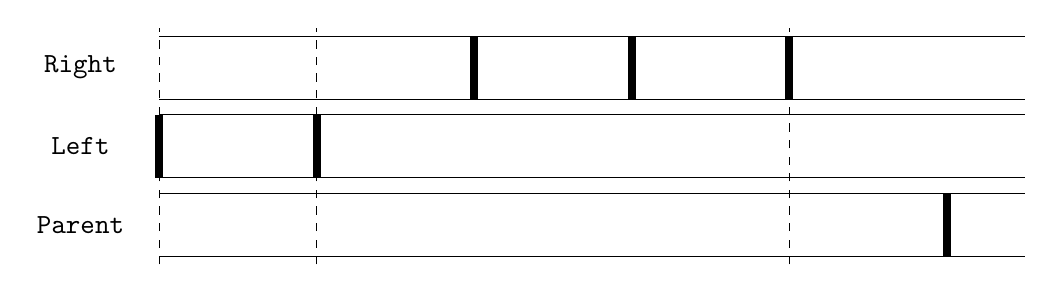
\begin{tikzpicture}
	\draw (0,2.9) -- (11,2.9);
	\draw (0,2.1) -- (11,2.1);
	\draw (0,1.9) -- (11,1.9);	
	\draw (0,1.1) -- (11,1.1);
	\draw (0,0.9) -- (11,0.9);
	\draw (0,0.1) -- (11,0.1);
	
	\vl{0}
	\vl{2}
	\vl{8}
	
	\draw[line width = 1mm] (0,1.1) -- (0,1.9);
	\draw[line width = 1mm] (2,1.1) -- (2,1.9);
	\draw[line width = 1mm] (8,2.1) -- (8,2.9);
	\draw[line width = 1mm] (4,2.1) -- (4,2.9);
	\draw[line width = 1mm] (6,2.1) -- (6,2.9);
	\draw[line width = 1mm] (10,0.1) -- (10,0.9);
	
	\node at (-1,0.5) {\tt Parent};
	\node at (-1,1.5) {\tt Left};
	\node at (-1,2.5) {\tt Right};
\end{tikzpicture}
\vspace{10mm}

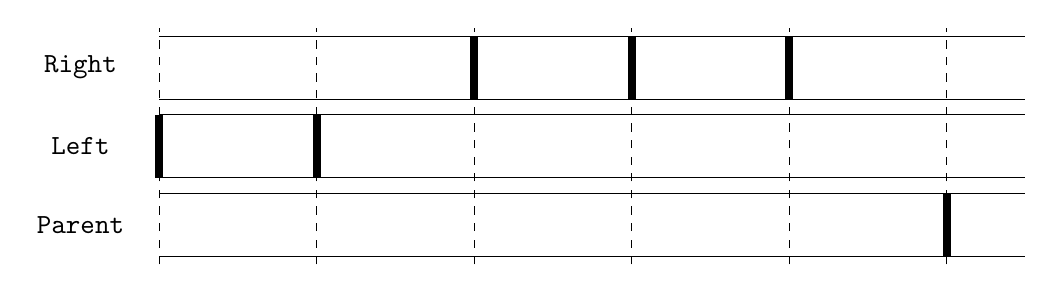
\begin{tikzpicture}
	\draw (0,2.9) -- (11,2.9);
	\draw (0,2.1) -- (11,2.1);
	\draw (0,1.9) -- (11,1.9);	
	\draw (0,1.1) -- (11,1.1);
	\draw (0,0.9) -- (11,0.9);
	\draw (0,0.1) -- (11,0.1);
	
	\vl{0}
	\vl{2}
	\vl{4}
	\vl{6}
	\vl{8}
	\vl{10}
	
	\draw[line width = 1mm] (0,1.1) -- (0,1.9);
	\draw[line width = 1mm] (2,1.1) -- (2,1.9);
	\draw[line width = 1mm] (8,2.1) -- (8,2.9);
	\draw[line width = 1mm] (4,2.1) -- (4,2.9);
	\draw[line width = 1mm] (6,2.1) -- (6,2.9);
	\draw[line width = 1mm] (10,0.1) -- (10,0.9);
	
	\node at (-1,0.5) {\tt Parent};
	\node at (-1,1.5) {\tt Left};
	\node at (-1,2.5) {\tt Right};
\end{tikzpicture}
\vspace{10mm}

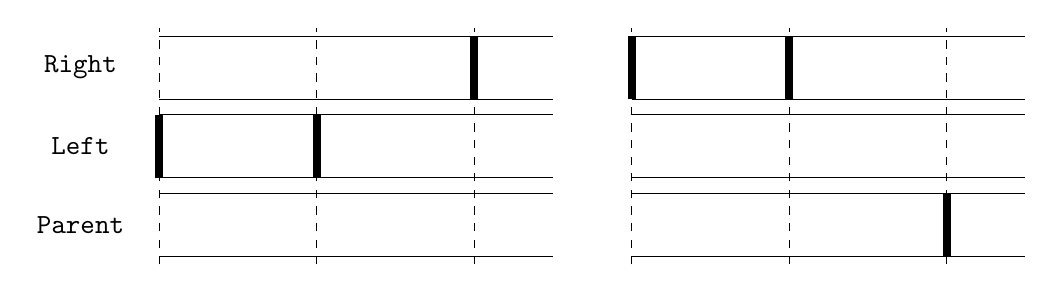
\begin{tikzpicture}
	\draw (0,2.9) -- (5,2.9);
	\draw (0,2.1) -- (5,2.1);
	\draw (0,1.9) -- (5,1.9);	
	\draw (0,1.1) -- (5,1.1);
	\draw (0,0.9) -- (5,0.9);
	\draw (0,0.1) -- (5,0.1);
	
	\draw (6,2.9) -- (11,2.9);
	\draw (6,2.1) -- (11,2.1);
	\draw (6,1.9) -- (11,1.9);	
	\draw (6,1.1) -- (11,1.1);
	\draw (6,0.9) -- (11,0.9);
	\draw (6,0.1) -- (11,0.1);
	
	\vl{0}
	\vl{2}
	\vl{4}
	\vl{6}
	\vl{8}
	\vl{10}
	
	\draw[line width = 1mm] (0,1.1) -- (0,1.9);
	\draw[line width = 1mm] (2,1.1) -- (2,1.9);
	\draw[line width = 1mm] (8,2.1) -- (8,2.9);
	\draw[line width = 1mm] (4,2.1) -- (4,2.9);
	\draw[line width = 1mm] (6,2.1) -- (6,2.9);
	\draw[line width = 1mm] (10,0.1) -- (10,0.9);
	
	\node at (-1,0.5) {\tt Parent};
	\node at (-1,1.5) {\tt Left};
	\node at (-1,2.5) {\tt Right};
\end{tikzpicture}
\vspace{10mm}
\end{center}
{
	\small
	One fat node is depicted in four stages of an update. Intervals of validity of its pointers are indicated by thick vertical lines. Beginning of a slot is illustrated by dashed vertical lines.

	In the topmost stage, no changes have been done to the fat node. In the second stage, we see that several fat nodes have been split and there are multiple fat nodes of {\tt Right} and {\tt Parent} corresponding to intervals of one slot. In the third stage we see that additional slots have been created. In the last stage, the fat node has been split in two.
}
\caption{An example of node splitting}
\end{figure}

We see that once $l$ is empty, no pointers are overlapping. Also capacity is not exceeded for no fat nodes. Now it is in order to show that $l$ will eventually become empty and what the time complexity is.

\begin{prop}
Starting with an initially empty fully-persistent binary search tree data structure (as described above), a sequence of $n$ updates produces a data structure taking \bigO{n} space while taking \bigO{n \log n} time.
\end{prop}

\begin{proof}
First of all we observe that the invariant restoring process of one vertex takes time linear with the amount of newly created fat nodes plus one and as such can be ignored.
	
Let us define a potential function for a persistent BST as the sum of potential energy stored in all of its fat nodes. 
Every fat node must always store at least as many units of potential as many slots it contains minus $m$. 
Initially (for empty tree) the potential is zero and may never be negative. One unit of potential can be used to allocate one fat node and execute constant number of other computation steps.

During the first phase, i.e. writing actual changes in the tree nodes, at most constant number of extra slots become occupied, the increase in potential from these insertions is charged on the update.

We also must analyze processing of fat nodes in $l$ during the second phase. Let us denote by $d$ the fat node that is being processed. 
During removal of overlapping pointers we add some slots, this must be covered in advance by transfer of potential from other vertices when these are split. 
If the node does not need to be split, constant amount of work was carried out. 
No additional pointers become overlapping, so no transfers of potential are required.

Otherwise for each newly created fat node overall potential of $d$ and its new successors is allowed to decrease by $m$.
This free potential is used to pay for allocation of new vertices (1 unit per new node). 
On top of that, some pointers may become overlapping. It can be seen that it suffices to transfer 1 unit to fat nodes which are pointed to by the first slot in a new fat node. Up to additional $p+k$ units are transferred to vertices which are pointed to by first slots in new fat nodes.
Identification of overlapping pointers is linear with number of new vertices linked after $d$.

From this argument we also see that the number of node-splitting occurring during one update is limited by the amount of potential available at the start of that update, so it must come to an end. Moreover constant amount is added to potential by updates in each operation, therefore space complexity is linear.

Every action is now accounted for and the proof is complete.
\end{proof}

\begin{cor}
A sequence of any $n$ tree-operations and $q$ queries on a fully persistent WAVL tree (initially empty) produces a data structure which consumes \bigO{n} memory and takes \bigO{(n+q) \log n} time.
\end{cor}

We should note that the size of vertices is so large, because we did not place any constraint on what updates are allowed to change. If update is only able to change one pointer field for example, we could reduce the size significantly. This would need to be analysed separately for each data structure.

One last thing we have not yet considered are pointers to the data structure from outside it. Surely, we need to store root for the tree in every version. For this purpose, we create a record with a pointer to a fat node together with the required version. Of course this by itself does not work, notably it does prevent the correct slot from leaving that fat node. 

This can be repaired by adding a special kind of pointer to slots indicating that there is a record  connected to this version of this vertex. When the fat node is then split, the record is updated with correct fat node. (This forces us to insert a slot to the root for each update though.) Pointers to other vertices can be achieved similarly.

\section{Alternative constructions}

In the previous section, we described fat nodes, where every slot bears all information about the tree vertex. There are other possibilities.

As was already mentioned, we may choose to have a set of default values for all fields and pointers.
These would be initialized to the first version in that fat vertex. Changes would then be stored in form of ordered triples. First would come version, second field or pointer identifier, and last the actual new value. Changing some information by adding a version thus means identifying what are the relevant values first and then inserting update triples.

Yet another option is similar to the last one with the difference that only updates of pointers are allowed. If field needs to be changed, new fat vertex must be allocated.

It is difficult to decide which of these constructions is superior. Complexity will vary for each data structure, ratios between different operations, and other factors.

Finally, let us conclude this chapter with a remark that this approach may be generalized further beyond binary search trees to other pointer-based data structures provided that the constraint on number of pointers targeting one node simultaneously applies to them.
We do not give more attention to such structures in this thesis.
